\documentclass[a4paper]{article}
\usepackage[spanish]{babel}
\usepackage[utf8]{inputenc}
% \usepackage{charter}   % tipografia
\usepackage[font=small,labelfont=bf]{caption}
\usepackage[font=small,labelfont=bf]{subcaption}
\usepackage{graphicx}
\usepackage{pdfpages}
\usepackage{float}
\usepackage{paralist} %itemize inline
\usepackage{amsmath, amsthm, amssymb}
\usepackage{underscore}
\usepackage{url}

% Tikz para dibujar grafiquitos
\usepackage{tikz}
\usetikzlibrary{babel}

\usepackage{pgfplots}
\pgfplotsset{width=12cm,height=6cm}

% Para pseudocodigo
\usepackage[linesnumbered,ruled,vlined]{algorithm2e}
\SetArgSty{textnormal}


% ********************************************************* %
% ~~~~~~~~         Formato de las páginas         ~~~~~~~~~ %
% ********************************************************* %

\usepackage{fancyhdr}
\pagestyle{fancy}

\renewcommand{\sectionmark}[1]{\markright{\thesection\ - #1}}

\fancyhf{}

\fancyhead[LO]{Sección \rightmark} % \thesection\ 
\fancyfoot[LO]{\small{Damián Fernando Huaier, Mateo Marenco, Daniel Matías Salvia, Ezequiel Togno}}
\fancyfoot[RO]{\thepage}
\renewcommand{\headrulewidth}{0.5pt}
\renewcommand{\footrulewidth}{0.5pt}
\setlength{\hoffset}{-0.8in}
\setlength{\textwidth}{16cm}
\setlength{\headsep}{0.5cm}
\setlength{\textheight}{25cm}
\setlength{\voffset}{-0.7in}
\setlength{\headwidth}{\textwidth}
\setlength{\headheight}{13.1pt}

\decimalpoint

\renewcommand{\baselinestretch}{1.1}  % line spacing

% ******************************************************** %


\begin{document}
\thispagestyle{plain}
%Esto es para algorithm2e
\DontPrintSemicolon

\centerline{\Large Universidad de Buenos Aires}
\vspace{2.5mm}
\centerline{\Large Facultad de Ciencias Exactas y Naturales}
\vspace{2.5mm}
\centerline{\Large Departamento de Computaci\'on}
\vspace{2.5mm}
\centerline{\Large Métodos Num\'ericos}
\vspace{12.5mm}
\centerline{\huge Reconstrucción de imágenes tomográficas}\par
\vspace{10mm}
\centerline{Huaier, Damián Fernando damianhuaier@gmail.com}
\centerline{Marenco, Mateo mateomarenco74@gmail.com}
\centerline{Salvia, Daniel Matías danmats140@gmail.com}
\centerline{Togno, Ezequiel ezetogno@gmail.com}
\vspace{10mm}

En este trabajo implementamos un método para reconstruir imágenes tomográficas. Dicho método busca aproximar las densidades de un objeto estudiado, 
atravesado por una cierta cantidad de rayos X. Disponiendo de los tiempos y las distancias recorridas por cada rayo se obtienen 
las densidades como una solución aproximada de un sistema de ecuaciones sobredeterminado. Dicha aproximación se realiza por \textit{cuadrados mínimos}.

En el presente informe se detalla el proceso de simulación tomográfico para generar datos de prueba, la implementación de cuadrados mínimos mediante 
la descomposición SVD, y la calidad de la imagen reconstruida en relación a la cantidad de rayos y la forma en que son generados, así como la manera 
en que se divide el objeto de estudio.

\vspace{0.5cm}

\noindent Palabras clave: \texttt{simulación tomográfica}, \texttt{cuadrados mínimos}, \texttt{SVD}

\newpage

\tableofcontents

\newpage

\setlength{\parskip}{0.2cm}

\newpage

\section{Introducción}

Nuestro objeto de estudio es, en teoría, un cuerpo continuo, cuadrado y bidimensional, con densidad variable en cada punto. Para reconstruir estas 
densidades primero se discretiza el cuerpo en cuestión, es decir, consideramos que está dividido en $n \times n$ celdas discretas. Los datos de 
entrada para nuestro método consisten, por cada rayo $k$ emitido sobre el cuerpo, en:

\begin{itemize}
\item El tiempo que tardó el rayo en atravesar el objeto, que llamaremos $t_k$.
\item La distancia que el rayo recorrió en cada celda $ij$, que llamaremos $d_{ij}^{(k)}$.
\end{itemize}

Para este trabajo consideraremos que la densidad en una celda $ij$ viene dada por $v_{ij}^{-1}$, que se entiende por la inversa de la velocidad con 
la que cualquier rayo atraviesa dicho punto. Teniendo en cuenta esto, notemos que para cada $k = 1 \ldots m$, siendo $m$ la cantidad de rayos, se 
tiene:

\[
\sum_{i=1}^n \sum_{j=1}^n d_{ij}^{(k)} v_{ij}^{-1} = t_k
\]

Si consideramos la matriz $D \in \mathbb{R}^{m \times n^2}$ que en cada fila $k$ posee todas las distancias $d_{ij}^{(k)}$ ordenadas primero por 
$i$ y después por $j$, y el vector $t = (t_1,\ldots,t_m)^t \in \mathbb{R}^m$, entonces el vector de intensidades de cada celda es una solución del 
sistema:

\[
Ds = t \ \ \ s \in \mathbb{R}^{n^2}
\]

Dado que no es posible medir el tiempo de los rayos sin errores, los tiempos $t_k$ traerán consigo cierto error, que será la causa de la imposibilidad 
de encontrar una solución exacta al sistema $Ds = t$. Por esta razón acudimos al método de cuadrados mínimos: se busca $s$ tal que minimice la cuenta 
$||Ds - t||^2$, o dicho de otra manera, buscamos el vector $s$ que más se ``parezca'' a una solución del sistema.

Este problema puede resolverse calculando la descomposición 
SVD\footnote{https://davidtabora.files.wordpress.com/2015/01/david_s-_watkins_fundamentals_of_matrix_computat.pdf. Página 262.} de la matriz $D$. 
Siendo $D = U\Sigma V^t$ dicha descomposición, podemos escribir:

\[
U^t t = 
    \begin{pmatrix}
      c \\
      d
    \end{pmatrix}
\]

\noindent con $c \in \mathbb{R}^{r}$, $d \in \mathbb{R}^{m - r}$ y $r = \text{rg}(D)$. Para hallar la solución primero se debe calcular el vector 
$y \in \mathbb{R}^{n^2}$ dado por:

\[
y = 
    \begin{pmatrix}
      c_1/\sigma_1 \\
      \vdots       \\
      c_r/\sigma_r \\
      y_{r+1}      \\
      \vdots       \\
      y_{n^2}      
    \end{pmatrix}
\]

\noindent con $\sigma_1 \ldots \sigma_r$ los valores singulares de $D$ y $y_{r+1} \ldots y_{n^2}$ arbitrarios. Finalmente se obtiene la solución 
$s = Vy$, que minimiza la norma $||Ds - t||^2$ y por lo tanto contendrá los valores aproximados de las densidades de todas las $n^2$ celdas del 
objeto \footnote{En el apéndice puede encontrarse una demostración de que una solución construida de esa manera es solución de cuadrados mínimos.}.

La calidad de la solución obtenida dependerá de la cantidad de rayos generados, de sus recorridos, del tamaño de la discretización y del nivel de 
ruido que posean los tiempos $t_k$. Analizaremos con detalle todos estos aspectos posteriormente, a partir de las experiencias realizadas.

Existe un inconveniente, y es que no se cuenta con datos provenientes de un tomógrafo real. Por lo tanto, en este trabajo trabajaremos con imágenes 
en escala de grises que representarán el objeto a estudiar. Los píxeles con intensidad más cercana a 255 (la máxima) indicarán zonas de mayor 
densidad y tendrán un color más claro, mientras que aquellos más cercanos a 0 (la mínima) se corresponderán con zonas de menor densidad y seran de 
un color más oscuro. Esta será una representación aproximada del cuerpo continuo y bidimensional que mencionamos anteriormente.

Una vez elegida dicha imagen se determina la discretización a utilizar, que consiste en decidir cuántos píxeles contendrá cada celda de la imagen.
Posteriormente se realiza una simulación de los rayos X: dado un rayo y una celda $ij$ calcularemos $d_{ij}^{(k)}$ como la cantidad de píxeles 
atravesados por el rayo en esa celda, es decir, consideramos que la distancia recorrida por cualquier rayo en cualquier pixel es 1. El tiempo que 
tarda en recorrer esa celda será entonces la suma de las intensidades de los píxeles tocados, resultado que será sumado al tiempo total $t_k$. Este 
proceso se realiza para todas las celdas.

Luego de realizar esta simulación añadiremos cierto nivel de ruido a todos los tiempos $t_k$, es decir, le sumaremos un valor aleatorio, para simular 
las imprecisiones que surgen de medir esta magnitud.

El objetivo general del trabajo es crear un programa en C++ que tome como dato de entrada una imagen en escala de grises, en formato \texttt{csv},
que represente el objeto a analizar, más una serie de parámetros que determinan la discretización a utilizar, la forma de generar los rayos, y 
el nivel de ruido. El programa realizará la simulación tomográfica y con los datos obtenidos reconstruirá la imagen. Esta nueva imagen será 
guardada en un \texttt{csv} de salida.

Como parte de la experiencia se analizará la calidad de la imagen reconstruida en relación a la imagen original, utilizando la métrica 
PSNR\footnote{http://www.ni.com/white-paper/13306/en/} ---Peak signal-to-noise ratio---, que se define como:

\[
\text{PSNR} = 10\cdot \log_{10}\left(\frac{\text{MAX}_u^2}{\text{ECM}}\right)
\]

\noindent donde $\text{MAX}_u$ es el rango máximo de la imagen, que en nuestro caso será 255, y ECM es el \textit{error cuadrático medio}:

\[
\text{ECM} = \frac{1}{N} \sum_{ij} (u_{ij}^{(0)} - u_{ij})^2
\]

\noindent siendo $u^{(0)}$ la imagen original, $u$ la imagen reconstruida y $N$ la cantidad de píxeles.




\newpage

\section{Desarrollo}

\subsection{Manejo de las imágenes}

Nuestro programa aceptará únicamente imágenes cuadradas en formato \texttt{csv}. Estas son representadas como un simple arreglo de arreglos de bytes. 
En caso de recibir una imagen cuyo tamaño no es divisible por el tamaño de las celdas especificado se presenta un problema puesto que no será posible 
dividir la misma en celdas cuadradas de manera exacta.

Una posible solución es extender la imagen con píxeles negros o de otra intensidad específica para que pueda ser discretizada. Sin embargo, si 
pensamos en las celdas que tendrán estos nuevos píxeles, su intensidad resultante luego de la reconstrucción puede llegar a ser muy influenciada 
por la presencia de dichos píxeles. Por lo tanto, decidimos que estos mismos posean distancia cero y que el tiempo en recorrerlos sea nulo. Es decir, 
directamente ignoramos su presencia. Visto de otra manera, lo que estamos haciendo es permitir que las celdas que no caben en la imagen sean no 
cuadradas para que sí lo hagan.

Una vez obtenida la imagen reconstruida, está será de menor tamaño que la original. Para poder obtener el PSNR decidimos agrandar la nueva imagen para 
que ambas tengan el mismo tamaño. Con el fin de estudiar la calidad de los resultados obtenidos únicamente con nuestro método de reconstrucción, la 
manera de agrandar la imagen no utilizará interpolación. El método será el más simple posible: cada píxel de ella, que se corresponde con una celda de 
la discretización, será dividido en tantos píxeles como los que tenía dicha celda, pero con la intensidad proveniente de la reconstrucción.

\subsection{Método de simulación de rayos}

Lo que haremos es pensar en la imagen original como un área del plano $\mathbb{R}^2$, pero el eje $y$ apuntará hacia abajo. %Por ejemplo, para una 
%imagen de $8\times 8$ píxeles definiremos el sistema de coordenadas de esta manera:
 
% \vspace{0.2cm}
% \begin{center}
% \begin{tikzpicture}[scale = 0.75]
% \draw [help lines] (0,1) grid (8,9);
% \draw [thick, <->] (9,9) -- (0,9) -- (0,0);
%\draw [thick, ->] (1,0.5) -- (1.75,0.5);
% \node [above] at (0,9) {0};
% \node [left] at (0,9) {0};
% \node [above] at (1,9) {1};
% \node [above] at (2,9) {2};
% \node [above] at (3,9) {3};
% \node [above] at (4,9) {4};
% \node [above] at (5,9) {5};
% \node [above] at (6,9) {6};
% \node [above] at (7,9) {7};
% \node [above] at (8,9) {8};
% \node [left] at (0,8) {1};
% \node [left] at (0,7) {2};
% \node [left] at (0,6) {3};
% \node [left] at (0,5) {4};
% \node [left] at (0,4) {5};
% \node [left] at (0,3) {6};
% \node [left] at (0,2) {7};
% \node [left] at (0,1) {8};
% \node [left] at (0,0) {$y$};
% \node [above right] at (9,9) {$x$};
% \end{tikzpicture}
% \end{center}
% \vspace{0.2cm}

Consideramos que para simular un rayo se deben especificar dos píxeles del borde de la imagen, $p_0 = (x_0,y_0)$ y $p_1 = (x_1,y_1)$. El rayo 
generado será una recta que pase por los centros de estos dos píxeles, es decir, por los puntos de $\mathbb{R}^2$ \ 
$\tilde{p_0} = (\tilde{x_0}, \tilde{y_0}) = (x_0 + 0.5, y_0 + 0.5)$ y 
$\tilde{p_1} = (\tilde{x_1}, \tilde{y_1}) = (x_1 + 0.5, y_1 + 0.5)$.

La idea es recorrer todos los píxeles que va atravesando la recta, y por cada uno de ellos sumamos su intensidad al tiempo total del rayo y 
además sumamos 1 a la distancia recorrida en la celda correspondiente.

La recta estará definida por la ecuación $y = f(x) = ax + b$ siendo 
$a = (\tilde{y_1} - \tilde{y_0})/(\tilde{x_1} - \tilde{x_0})$ y $b = \tilde{y_0} - a \tilde{x_0}$.

Como pixel de inicio se eligirá entre $p_0$ y $p_1$ a aquel que esté más a la izquierda. Para ver como se recorren los píxeles, llamemos $(x,y)$ 
a las coordenadas (enteras) de este pixel. Lo que haremos es evaluar nuestra función $f$ en el borde derecho del pixel, es decir, obtendremos 
$f(x+1)$ y en base a su resultado tomaremos los siguientes caminos:

\begin{itemize}
\item $f(x+1) < y$: pasar al pixel de arriba.
\item $f(x+1) = y$: pasar al pixel que está arriba y hacia la derecha.
\item $y < f(x+1) < y+1$: pasar al píxel de la derecha.
\item $f(x+1) = y+1$: pasar al pixel que está abajo y hacia la derecha.
\item $y+1 < f(x+1)$: pasar al píxel de abajo.
\end{itemize}

% \begin{tikzpicture}[scale = 0.6]
% \fill [blue] (0,1) rectangle (1,2);
% \fill [blue] (0,2) rectangle (1,3);
% \draw [help lines] (-1,0) grid (3,5);
% \draw [white] (-1,0) rectangle (3,5);
% \draw [thick] (-1,4.1) -- (3,3);
% \end{tikzpicture}
% \hspace{1.0cm}
% \begin{tikzpicture}[scale = 0.6]
% \fill [blue] (0,2) rectangle (1,3);
% \fill [blue] (1,2) rectangle (2,3);
% \draw [help lines] (0,0) grid (3,5);
% \draw [white] (0,0) rectangle (3,5);
% \end{tikzpicture}
% \hspace{1.0cm}
% \begin{tikzpicture}[scale = 0.6]
% \fill [blue] (0,2) rectangle (1,3);
% \fill [blue] (0,1) rectangle (1,2);
% \draw [help lines] (0,0) grid (3,5);
% \draw [white] (0,0) rectangle (3,5);
% \end{tikzpicture}

Es decir, no hacemos más que saltar al pixel que sea tocado por el rayo. Este proceso se repite hasta que detectemos que ya no estamos más parados 
en el área de $\mathbb{R}^2$ ocupada por la imagen.

Si el rayo es vertical, es decir $x_0 = x_1$, entonces los puntos exactos por los que pasa la recta, $\tilde{p_0}$ y $\tilde{p_1}$, serán ligeramente 
corridos (uno hacia la izquierda y el otro hacia la derecha) de manera que la recta quede levemente ``torcida'' y así poder calcular los coeficientes 
$a$ y $b$ de la recta, pero evitando que la misma colisione con píxeles de más.

El nivel de ruido será especificado por una constante positiva $R$. Luego de simular cada rayo y obtener el tiempo $t_k$, a este valor se le sumará 
un número aleatorio en el intervalo $[-R,R]$.

\subsection{Representación de matrices}

Es claro que la cantidad de píxeles que atraviesa un rayo es escasa en comparación con la cantidad total de píxeles de la imagen. Si la imagen  
tiene $\ell \times \ell$ píxeles podemos esperar que cada rayo atraviese $\ell$ píxeles aproximadamente. Como consecuencia tendremos que para cada $k$ 
habrá muchos $d_{ij}^{(k)}$ nulos, y por lo tanto la matriz $D$ será muy rala.

La decisión más razonable es guardar solo los elementos no nulos de $D$ para utilizar menos memoria y agilizar los cálculos que se deberán 
realizar posteriormente. Lo que haremos entonces es representar a $D$ como un arreglo de vectores ralos, donde cada vector ralo representa 
una columna de la matriz. Por su parte un vector ralo se representa como un arreglo de pares, donde cada par contiene un valor no nulo del 
vector y la posición de este en el vector. Estos pares están ordenados en orden creciente de acuerdo a las posiciones.

La decisión de representar las columnas de $D$ con vectores ralos, en vez de las filas, tiene la siguiente motivación: sabiendo que para 
la descomposición SVD calcularemos la matriz $D^t D$ y que $(D^t D)_{ij}$ se calcula como el producto interno entre la columna $i$ y la columna 
$j$ de $D$, estos productos internos serán obtenidos con mucha rapidez si las columnas son vectores ralos.

Sin embargo, no hay garantías de que $D^t D$ resulte rala, por lo tanto dicha matriz será representada como un arreglo de arreglos de 
\texttt{double}'s. Lo mismo vale para el resto de las matrices que se deban calcular.

\subsection{Cálculo de autovalores y autovectores}

La descomposición SVD requerirá la obtención de los autovalores y autovectores de $D^t D$. Para llevar a cabo esta tarea utilizaremos el 
\textit{método de la potencia con deflación}, aplicable a matrices con base de autovectores ortogonales, como $D^tD$. En primer lugar consideramos 
un vector $v_0$ arbitrario y la sucesión:

\[
v_{k+1} = \frac{D^tD v_k}{||D^tD v_k||}
\]

\noindent para hallar el autovector asociado al autovalor de mayor magnitud $\lambda$, que a su vez puede calcularse como $\lambda = v^tD^tDv$ 
siendo $v$ el autovector obtenido. Una vez obtenidos $v$ y $\lambda$ se procede a calcular la matriz $D^tD - \lambda v v^t$, a la cual se le 
aplica nuevamente el método de la potencia para hallar el segundo autovalor y autovector dominante de $D^tD$. Este proceso se sigue repitiendo 
hasta hallar todos los autovectores y autovalores.

Es claro que este método puede llegar a ser muy inestable puesto que cada autovalor $\lambda$ y autovector $v$ que hallemos 
tendrán un cierto error, debido a cuestiones numéricas y a que quizás no se realizó una cantidad de iteraciones suficiente. Por más que sea 
aceptable, dicho error se trasladará al cálculo de la nueva matriz durante el paso de la deflación, y por lo tanto los siguientes autovalores 
y autovectores tendrán aún más error.

Para lidiar con esta situación decidimos adoptar el siguiente criterio de convergencia: la iteración termina cuando el vector actual $v_k$ está 
lo suficientemente cerca de ser un autovector de $D^tD$, es decir, cuando:

\[
E_k = \frac{||D^tDv_k - \lambda_k v_k||}{||\lambda_k v_k||} \leq \varepsilon_1
\]

\noindent con $\lambda_k = v_k^tD^tDv_k$ y $\varepsilon_1$ una constante global. Es importante remarcar que esta condición se prueba utilizando 
$D^tD$ en vez de la matriz actual a la que le estemos aplicando el método de la potencia. Esto asegurará que todos los autovectores y autovalores 
sean igual de precisos que los primeros.

Debido a que con este criterio puede ocurrir que el error $E_k$ nunca llegue a ser menor o igual a $\varepsilon_1$, nuestra implementación detecta 
esta situación, viendo que $E_k = E_{k-1}$ (es decir, luego de una iteración el error no mejoró) y en ese caso devuelve el autovalor y autovector 
actual tal como si el criterio se hubiera cumplido. Si $E_k$ era casi menor o igual a $\varepsilon_1$ entonces el resultado devuelto será aceptable 
y típicamente no se volverá a repetir la misma situación durante el cálculo de los próximos autovalores y autovectores (esto puede ser corroborado 
experimentalmente).

Sin embargo, si $E_k$ es demasiado alto (mayor a otra constante global más grande que $\varepsilon_1$, llamada $\varepsilon_2$) entonces nuestra 
implementación frenará el cálculo de todos los autovalores y autovectores. Además, también se frenará si un autovalor resultó mucho más grande que 
el anterior, o si un autovalor dio negativo. Esta última condición está impuesta porque $D^t D$ es semi-definida positiva y por lo tanto sus 
autovalores son no negativos. 

Notemos que en esos casos frenar todo el cálculo es lo más sensato, ya que si no lo hacemos los próximos autovalores y autovectores ya no serán 
válidos puesto que en la deflación habremos usado un $\lambda$ y un $v$ erróneos.

Para concluir esta sección se describe en el Algoritmo \ref{alg:maineig} el método propuesto, siendo $A$ la matriz a la cual calcularle el autovalor de mayor magnitud 
$\lambda$ junto con su autovector asociado $v$, y siendo $A_0$ la matriz con la cual se computará el error $E_k$ en cada iteración. El vector $v_0$ 
es el vector inicial con el cual se empieza a iterar, y la variable $outcome$ es un indicador de qué tan buenos fueron los resultados.

\vspace{\baselineskip}
\begin{algorithm}[H]
    \KwIn{$A$, $v_0$, $A_0$}
    \KwOut{$\lambda$, $v$, $outcome$}
    $v \gets v_0$\;
    \For{$k = 1 \ldots$}{
        \For{$i = 1 \ldots N$}{
            $v \gets \frac{Av}{||Av||}$\;
        }
        
        $\lambda \gets v^tAv$\;
        $E_k \gets \frac{||A_0 v - \lambda v||}{||\lambda v||}$\;
        \uIf{$E_k \leq \varepsilon_1$}{
            $outcome \gets$ ``Resultado aceptable''\;
            \Return{$\lambda$, $v$, $outcome$}
        }
        \ElseIf{$E_k = E_{k-1}$}{
            \uIf{$E_k \leq \varepsilon_2$}{
                $outcome \gets$ ``Resultado casi aceptable''\;
            }
            \Else{
                $outcome \gets$ ``Resultado inaceptable''\;
                
            }
            \Return{$\lambda$, $v$, $outcome$}
        }
    }
    \caption{Cálculo de autovalor y autovector dominante.}
    \label{alg:maineig}
\end{algorithm}
\vspace{\baselineskip}

Notemos que la instrucción $v \gets \frac{Av}{||Av||}$ se ejecuta una cantidad de veces $N$ antes de evaluar si seguir iterando o no. Esto genera 
que se gaste menos tiempo calculando el error $E_k$, el cual requiere una multiplicación de matriz por vector adicional ($A_0 v$).

Nuestra implementación fija los valores $N = 25$, $\varepsilon_1 = 0.01$, y $\varepsilon_2 = 0.1$. Notemos que 0.01 no es un límite muy exigente 
para $\varepsilon_1$, sin embargo, gracias a que el error se mide utilizando la matriz original, los resultados son bastante aceptables, y al poder 
utilizar un límite no tan exigente el método termina haciendo menos iteraciones y por lo tanto se mejora el rendimiento. Si midiéramos el error 
usando la matriz actual (en el caso del Algoritmo \ref{alg:maineig}, se trata de la matriz $A$) tendríamos que reducir el valor de $\varepsilon_1$ 
y por lo tanto el tiempo de procesamiento sería mayor.

Con esta función se calculan todos los autovectores y autovalores de $D^tD$ que sean posibles. Los chequeos de signo y magnitud de los autovalores 
devueltos, mencionados anteriormente, son llevados a cabo por fuera de esta función.

\subsection{Descomposición SVD y cuadrados mínimos}

Según se mencionó en la introducción, obtener la solución de cuadrados mínimos resulta muy sencillo conociendo la factorización SVD de la matriz 
$D$.

Para obtener esta descomposición decidimos calcular $D^t D$ en vez de $DD^t$ porque la primera será de tamaño $n^2 \times n^2$ y la segunda 
de $m \times m$, y típicamente la cantidad de rayos $m$ será mayor a la cantidad de celdas $n^2$, por lo tanto $D^t D$ será más chica.
Su cálculo consiste en realizar los productos internos entre las columnas de D para determinar cada $(D^t D)_{ij}$. Esto se hace solo para 
$i \leq j$, puesto que $(D^t D)_{ij} = (D^t D)_{ji}\ \forall i,j$. Los productos internos serán más rápidos de lo normal gracias a que 
las columnas son vectores ralos.

Una vez obtenida $D^t D$ se procede a calcular sus autovalores y autovectores. Los autovectores serán las columnas $v_1 \ldots v_n$ de $V$ y 
las raíces cuadradas de los autovalores (que serán positivos puesto que $D^t D$ es semi-definida positiva) serán los valores singulares 
$\sigma_1 \ldots \sigma_r$ con $r = \text{rg}(D)$.

Si recordamos lo que se mencionó en la introducción, podemos deducir que solo nos interesan las primeras $r$ filas de $U^t$, ya que el resto 
de las filas solo importan para el resultado del vector $d$, que no utilizamos. Entonces podemos usar que, para todo $i$ entre $1$ y $r$:

\[
D v_i = \sigma_i u_i
\]
\[
\implies u_i = D v_i / \sigma_i
\]

Esto nos brinda un método sencillo y eficaz para calcular las filas de $U^t$ que nos importan. Calcular $D v_i$ en principio parece complicado 
al no poder operar fácilmente con las filas de $D$. Sin embargo, podemos pensar que $D v_i$ es una combinación lineal de las columnas de $D$,
donde los coeficientes son los elementos de $v_i$. Aprovechando que las columnas son vectores ralos resulta fácil optimizar el cálculo de 
esta combinación lineal.

Una vez obtenidas $U^t$ y $V$ y los valores singulares, se procede a calcular el vector $c = U^t t$, con el cual obtendremos el vector $y$ 
según figura en la introducción. Los valores $y_{r+1} \ldots y_n$ son arbitrarios, puesto que cualquier elección dará lugar a una solución 
de cuadrados mínimos (es decir, las soluciones son infinitas, justamente porque $r = \text{rg}(D) < n$). Por convención, decidimos dejar todos 
ellos como cero. La solución final se obtiene haciendo el producto $s = Vy$, que puede entenderse como una combinación lineal de las columnas de 
$V$.

Existe un problema, y es que es posible que no obtengamos todos los autovalores y autovectores de $V$, según nuestra implementación del 
método de la potencia. En este caso lo que hacemos es quedarnos con los $\ell$ autovalores y autovectores que hayamos podido calcular, y en 
este caso las matrices $U$ y $V$ serán más chicas y dispondremos solamente de $\ell$ valores singulares. Como consecuencia los vectores 
$c$ e $y$ no tendrán $r$ elementos si no $\ell$, y el resultado final será una combinación lineal de las $\ell$ columnas de $V$.

Visto de otra manera, lo que sucede es que obtenemos una combinación lineal de no todas las columnas de la verdadera matriz $V$, puesto que 
las otras no las tenemos porque no las hemos podido calcular. Si las columnas que faltan son solo unas pocas podemos esperar que el 
resultado $s$ sea más o menos aceptable.

Durante este proceso también calcularemos $\kappa(D^tD)$, el número de condición de $D^tD$. Dado que esta matriz es simétrica y semi-definida 
positiva sus autovalores, que ya habremos calculado, serán iguales a sus valores singulares. Sabiendo que el número de condición se puede calcular 
como el valor singular más grande dividido el más chico, $\kappa(D^tD)$ será obtenido dividiendo su autovalor más grande por el más chico.

El número de condicion de $D^tD$ resulta de particular interés ya que toda solución de cuadrados mínimos del sistema $Ds = t$ es solución de las 
\textit{ecuaciones normales}:

\[
D^tDs = D^tt
\]

Cuanto más cercano a 1 sea $\kappa(D^tD)$, más estable será la solución obtenida. Por otro lado, si $\kappa(D^tD)$ es muy grande la solución será 
muy inestable y la matriz estará más cerca de ser singular. En efecto, si la matriz es singular entonces el autovalor más chico será cero y el número 
de condición no podrá calcularse. Este viene a ser el peor escenario en cuanto a estabilidad.

Por lo tanto una condición necesaria para no caer en este caso es que $D^tD$ sea inversible, lo que es equivalente a pedir que $D^tD$ sea SDP (ya que 
sabemos que es simétrica semi-definida positiva), a que la solución de las ecuaciones normales sea única, y a que la solución de cuadrados mínimos de 
$Ds = t$ sea única. Esta última condición es equivalente a que las columnas de $D$ sean linealente independientes, y su cumplimiento o no dependerá 
de la discretización utilizada y principalmente de la forma de generar los rayos.

\subsection{Hipótesis sobre los resultados}

En primer lugar, es claro que cuanto menor sea el tamaño de las celdas, mayor será la calidad de la reconstrucción. Sin embargo resulta difícil 
trabajar con tantas celdas debido al tiempo de ejecución, puesto que la matriz $D^tD$ será muy grande. Esto no solo implica que se deberán hallar 
más autovalores, si no que además las iteraciones del metodo de la potencia serán más costosas. Dependiendo del contexto de uso se puede discretizar 
el cuerpo en partes muy grandes para priorizar el rendimiento, o bien se puede optar por obtener una reconstrucción de mayor calidad dividiendo el 
cuerpo en partes más pequeñas.

Por otro lado, más allá del tamaño de celda elegido, no cualquier forma de generar los rayos resultará efectiva. Lo mínimo que se debe pedir para 
obtener una solución estable es que la cantidad de rayos sea mayor a la cantidad de celdas, es decir, que $D$ tenga más filas que columnas, y que 
además toda celda sea atravesada por al menos un rayo. Si cualquiera de esas dos condiciones no se cumplen entonces las columnas de $D$ no serán l.i.
Sin embargo, esto no garantiza que, en caso de cumplirse, sean l.i.

Resulta difícil imaginarse una forma de generar rayos que garantice independencia lineal. Lo mejor que se puede hacer es generar la mayor cantidad de 
rayos posibles, en diversas direcciones, de manera aleatoria o no.

También es importante que no solo cada celda sea atravesada por al menos un rayo. Se necesita que sea atravesada por varios rayos que en conjunto 
logren pasar por todos sus píxeles. Si hay píxeles que no son atravesados estaremos descartando la información que aportan, al momento de reconstruir 
la imagen.

Con respecto al rendimiento, la cantidad de rayos generados influirá en tres partes de nuestra implementación: la simulación tomográfica, el cálculo 
de $D^tD$, y la obtención de las filas de $U^t$. Si estamos trabajando con imágenes muy grandes deberemos ser cuidadosos a la hora de elegir la forma 
de generar los rayos puesto que podríamos generar un \textit{bottleneck}. De más está decir que, si se tratara de un caso real, habría un límite en 
la cantidad de radiación a generar ya que esta puede ser altamente nociva.

Por último, un parámetro más a tener en cuenta es el nivel de ruido que se agregará a los tiempos $t_k$. Naturalmente, a mayor cantidad de ruido, peor 
será la calidad de la imagen reconstruida, y más aún si el número de condición de $D^tD$ es muy alto. Sin embargo no tendrá efecto alguno en el 
rendimiento. De hecho, nuestra implementación permite realizar todo el proceso de simulación y reconstrucción para varios niveles de ruido a la vez.

\subsection{Propuesta de experimentación}

En primer lugar experimentaremos con diferentes tamaños de celda para las imágenes \texttt{tomo2.csv} y \texttt{tomo3.csv}, de tamaño 
$549 \times 549$ y $452 \times 452$ píxeles respectivamente. En la Figura \ref{fig:tomo23} mostramos ambas imágenes pero en sus tamaños originales,
donde no son cuadradas.

\begin{figure}
\centering
\begin{subfigure}{0.5\textwidth}
  \centering
  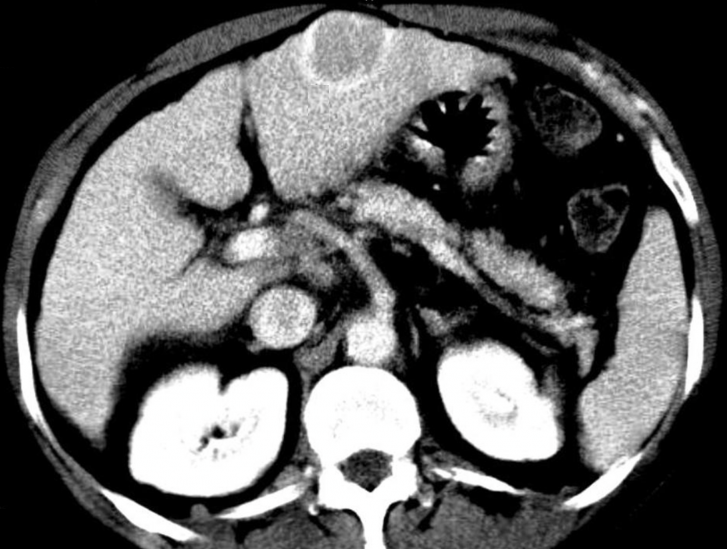
\includegraphics[width=0.8\linewidth]{tomo2}
  \caption{\texttt{tomo2}}
  \label{fig:sub1}
\end{subfigure}%
\begin{subfigure}{0.5\textwidth}
  \centering
  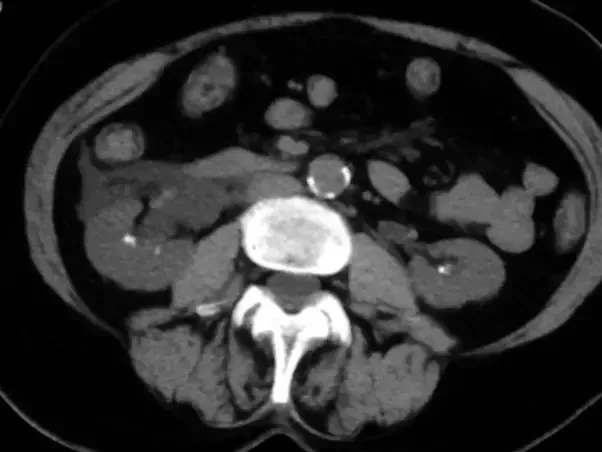
\includegraphics[width=0.8\linewidth]{tomo3}
  \caption{\texttt{tomo3}}
  \label{fig:sub2}
\end{subfigure}
\caption{Imágenes de prueba \texttt{tomo2} y \texttt{tomo3}.}
\label{fig:tomo23}
\end{figure}

\begin{figure}
\centering
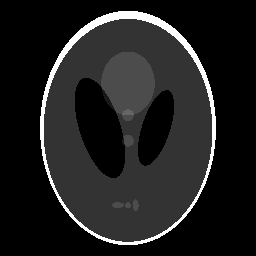
\includegraphics[width=0.3\linewidth]{phantom}
\caption{Imagen de prueba \texttt{phantom.csv}.}
\label{fig:phantom}
\end{figure}

\begin{figure}
\centering
\begin{tikzpicture}[scale = 0.5]
% \draw [help lines] (0,0) grid (10,10);
\draw [thick] (0,0) rectangle (10,10);

\draw [ultra thin] (0,0.5) -- (10,0.5);
\draw [ultra thin] (0,1.5) -- (10,1.5);
\draw [ultra thin] (0,2.5) -- (10,2.5);
\draw [ultra thin] (0,3.5) -- (10,3.5);
\draw [ultra thin] (0,4.5) -- (10,4.5);
\draw [ultra thin] (0,5.5) -- (10,5.5);
\draw [ultra thin] (0,6.5) -- (10,6.5);
\draw [ultra thin] (0,7.5) -- (10,7.5);
\draw [ultra thin] (0,8.5) -- (10,8.5);
\draw [ultra thin] (0,9.5) -- (10,9.5);

\draw [ultra thin] (0.5,0) -- (0.5,10);
\draw [ultra thin] (1.5,0) -- (1.5,10);
\draw [ultra thin] (2.5,0) -- (2.5,10);
\draw [ultra thin] (3.5,0) -- (3.5,10);
\draw [ultra thin] (4.5,0) -- (4.5,10);
\draw [ultra thin] (5.5,0) -- (5.5,10);
\draw [ultra thin] (6.5,0) -- (6.5,10);
\draw [ultra thin] (7.5,0) -- (7.5,10);
\draw [ultra thin] (8.5,0) -- (8.5,10);
\draw [ultra thin] (9.5,0) -- (9.5,10);

\draw [ultra thin] (8,0) -- (10,2);
\draw [ultra thin] (7,0) -- (10,3);
\draw [ultra thin] (6,0) -- (10,4);
\draw [ultra thin] (5,0) -- (10,5);
\draw [ultra thin] (4,0) -- (10,6);
\draw [ultra thin] (3,0) -- (10,7);
\draw [ultra thin] (2,0) -- (10,8);
\draw [ultra thin] (1,0) -- (10,9);
\draw [ultra thin] (0,0) -- (10,10);
\draw [ultra thin] (0,1) -- (9,10);
\draw [ultra thin] (0,2) -- (8,10);
\draw [ultra thin] (0,3) -- (7,10);
\draw [ultra thin] (0,4) -- (6,10);
\draw [ultra thin] (0,5) -- (5,10);
\draw [ultra thin] (0,6) -- (4,10);
\draw [ultra thin] (0,7) -- (3,10);
\draw [ultra thin] (0,8) -- (2,10);

\draw [ultra thin] (0,2) -- (2,0);
\draw [ultra thin] (0,3) -- (3,0);
\draw [ultra thin] (0,4) -- (4,0);
\draw [ultra thin] (0,5) -- (5,0);
\draw [ultra thin] (0,6) -- (6,0);
\draw [ultra thin] (0,7) -- (7,0);
\draw [ultra thin] (0,8) -- (8,0);
\draw [ultra thin] (0,9) -- (9,0);
\draw [ultra thin] (0,10) -- (10,0);
\draw [ultra thin] (1,10) -- (10,1);
\draw [ultra thin] (2,10) -- (10,2);
\draw [ultra thin] (3,10) -- (10,3);
\draw [ultra thin] (4,10) -- (10,4);
\draw [ultra thin] (5,10) -- (10,5);
\draw [ultra thin] (6,10) -- (10,6);
\draw [ultra thin] (7,10) -- (10,7);
\draw [ultra thin] (8,10) -- (10,8);

\end{tikzpicture}
\hspace{1.0cm}
\begin{tikzpicture}[scale=0.5]
\draw [thick] (0,0) rectangle (10,10);

\draw [ultra thin] (0,0) -- (1,10);
\draw [ultra thin] (0,0) -- (2,10);
\draw [ultra thin] (0,0) -- (3,10);
\draw [ultra thin] (0,0) -- (4,10);
\draw [ultra thin] (0,0) -- (5,10);
\draw [ultra thin] (0,0) -- (6,10);
\draw [ultra thin] (0,0) -- (7,10);
\draw [ultra thin] (0,0) -- (8,10);
\draw [ultra thin] (0,0) -- (9,10);
\draw [ultra thin] (0,0) -- (10,10);
\draw [ultra thin] (0,0) -- (10,9);
\draw [ultra thin] (0,0) -- (10,8);
\draw [ultra thin] (0,0) -- (10,7);
\draw [ultra thin] (0,0) -- (10,6);
\draw [ultra thin] (0,0) -- (10,5);
\draw [ultra thin] (0,0) -- (10,4);
\draw [ultra thin] (0,0) -- (10,3);
\draw [ultra thin] (0,0) -- (10,2);
\draw [ultra thin] (0,0) -- (10,1);

\draw [ultra thin] (10,0) -- (10,10);
\draw [ultra thin] (10,0) -- (9,10);
\draw [ultra thin] (10,0) -- (8,10);
\draw [ultra thin] (10,0) -- (7,10);
\draw [ultra thin] (10,0) -- (6,10);
\draw [ultra thin] (10,0) -- (5,10);
\draw [ultra thin] (10,0) -- (4,10);
\draw [ultra thin] (10,0) -- (3,10);
\draw [ultra thin] (10,0) -- (2,10);
\draw [ultra thin] (10,0) -- (1,10);
\draw [ultra thin] (10,0) -- (0,10);
\draw [ultra thin] (10,0) -- (0,9);
\draw [ultra thin] (10,0) -- (0,8);
\draw [ultra thin] (10,0) -- (0,7);
\draw [ultra thin] (10,0) -- (0,6);
\draw [ultra thin] (10,0) -- (0,5);
\draw [ultra thin] (10,0) -- (0,4);
\draw [ultra thin] (10,0) -- (0,3);
\draw [ultra thin] (10,0) -- (0,2);
\draw [ultra thin] (10,0) -- (0,1);
\draw [ultra thin] (10,0) -- (0,0);

\draw [ultra thin] (0,10) -- (10,10);
\draw [ultra thin] (0,10) -- (10,9);
\draw [ultra thin] (0,10) -- (10,8);
\draw [ultra thin] (0,10) -- (10,7);
\draw [ultra thin] (0,10) -- (10,6);
\draw [ultra thin] (0,10) -- (10,5);
\draw [ultra thin] (0,10) -- (10,4);
\draw [ultra thin] (0,10) -- (10,3);
\draw [ultra thin] (0,10) -- (10,2);
\draw [ultra thin] (0,10) -- (10,1);
\draw [ultra thin] (0,10) -- (10,0);
\draw [ultra thin] (0,10) -- (9,0);
\draw [ultra thin] (0,10) -- (8,0);
\draw [ultra thin] (0,10) -- (7,0);
\draw [ultra thin] (0,10) -- (6,0);
\draw [ultra thin] (0,10) -- (5,0);
\draw [ultra thin] (0,10) -- (4,0);
\draw [ultra thin] (0,10) -- (3,0);
\draw [ultra thin] (0,10) -- (2,0);
\draw [ultra thin] (0,10) -- (1,0);
\draw [ultra thin] (0,10) -- (0,0);

\draw [ultra thin] (10,10) -- (0,10);
\draw [ultra thin] (10,10) -- (0,9);
\draw [ultra thin] (10,10) -- (0,8);
\draw [ultra thin] (10,10) -- (0,7);
\draw [ultra thin] (10,10) -- (0,6);
\draw [ultra thin] (10,10) -- (0,5);
\draw [ultra thin] (10,10) -- (0,4);
\draw [ultra thin] (10,10) -- (0,3);
\draw [ultra thin] (10,10) -- (0,2);
\draw [ultra thin] (10,10) -- (0,1);
\draw [ultra thin] (10,10) -- (0,0);
\draw [ultra thin] (10,10) -- (1,0);
\draw [ultra thin] (10,10) -- (2,0);
\draw [ultra thin] (10,10) -- (3,0);
\draw [ultra thin] (10,10) -- (4,0);
\draw [ultra thin] (10,10) -- (5,0);
\draw [ultra thin] (10,10) -- (6,0);
\draw [ultra thin] (10,10) -- (7,0);
\draw [ultra thin] (10,10) -- (8,0);
\draw [ultra thin] (10,10) -- (9,0);
\draw [ultra thin] (10,10) -- (10,0);

\end{tikzpicture}
\caption{Rayos horizontales, verticales y diagonales (izquierda), y rayos que barren la imagen (derecha).}
\end{figure}

Como nuestro objetivo será estudiar cómo varía tanto la calidad según 
nuestra apreciación subjetiva como el valor del PSNR en función del tamaño de celda, dejaremos fijos el método de generación de rayos y el nivel de 
ruido. El primero será un método con el cual se generan 20000 rayos aleatorios (será descripto en breve), y el nivel de ruido será de 0.0. Además, 
veremos si el tamaño de celda influye en el número de condición $\kappa(D^tD)$.

Por otro lado, para las imágenes \texttt{tomo2.csv}, \texttt{phantom.csv} (mostrada en la Figura \ref{fig:phantom}) y \texttt{tomo.csv} (igual a 
\texttt{tomo2} pero redimensionada a $100 \times 100$ píxeles) probaremos los siguientes métodos de generación de rayos:

\begin{itemize}
\item Rayos verticales, horizontales y diagonales: consiste en generar todos los rayos posibles que sean horizontales, verticales y diagonales 
con pendiente 1.
\item Rayos que barren la imagen: consite en pararse en cada una de las cuatro esquinas de la imagen y desde ese punto generar rayos que vayan 
a todos los píxeles del borde (exceptuando los bordes que comparten dicho punto).
\item Rayos aleatoros: dada una cantidad de rayos deseada $m$, cada rayo aleatorio se genera de la siguiente manera:
\begin{itemize}
\item Se elige aleatoriamente si el rayo viajará del borde superior al inferior, del izquierdo al derecho, del superior al derecho, del derecho 
al inferior, del inferior al izquierdo o del izquierdo al superior.
\item Se eligen dos puntos aleatorios, uno de cada borde elegido, que determinarán el rayo.
\end{itemize}
\item Método ``completo'': se generan todos los rayos posibles que pasen por dos píxeles que vivan en bordes opuestos de la imagen.
\end{itemize}

Por último tomaremos la imagen \texttt{tomo2.csv} y estudiaremos el PSNR obtenido en función del nivel de ruido agregado, así como la calidad 
de la imagen reconstruida para algunos niveles de ruido, con el objetivo de medir el impacto que tiene este parámetro.

\clearpage

\section{Resultados}

En las figuras mostramos los diversos resultados obtenidos según la propuesta de experimentación.

Los resultados obtenidos con el método de rayos horizontales, verticales y diagonales son los siguientes:

\begin{itemize}
\item \texttt{phantom.csv}: PSNR = 15.2316.
\item \texttt{tomo3.csv}: PSNR = 17.0948.
\end{itemize}

Con el método de barridos:

\begin{itemize}
\item \texttt{phantom.csv}: PSNR = 12.4005
\item \texttt{tomo3.csv}: PSNR = 13.9602
\end{itemize}


%------------ PSNR en funcion de tamaño de celda ------------%

\begin{figure}[h]
\centering
\begin{tikzpicture}
\begin{axis}[
    title={PSNR en función del tamaño de celda},
    xlabel={Tamaño de celda},
    ylabel={PSNR},
    xmin=10, xmax=20,
    ymin=14, ymax=23,
    xtick={10,11,12,13,14,15,16,17,18,19,20},
    ytick={14,15,16,17,18,19,20,21,22,23},
    legend pos=north east,
    ymajorgrids=true,
    xmajorgrids=true,
    grid style=dashed,
]

\addplot[
    color=blue,
    mark=*,
    style=dashed,
    ]
    coordinates {
    (20,14.2203)
    (19,14.4431)
    (18,14.584)
    (17,14.9159)
    (16,15.1494)
    (15,15.5134)
    (14,15.7002)
    (13,15.9758)
    (12,16.466)
    (11,16.8652)
    (10,17.2959)
    };
    \addlegendentry{\texttt{tomo2.csv}}

\addplot[
    color=red,
    mark=*,
    style=dashed,
    ]
    coordinates {
    (10,22.4565)
    (11,22.1921)
    (12,21.7393)
    (13,21.4325)
    (14,20.7527)
    (15,20.4585)
    (16,20.4911)
    (17,20.2983)
    (18,19.7594)
    (19,19.6317)
    (20,19.6563)
    };
    \addlegendentry{\texttt{tomo3.csv}}

\end{axis}
\end{tikzpicture}
\caption{PSNR en función del tamaño de celda, para las imágenes \texttt{tomo2.csv} y \texttt{tomo3.csv}. Nivel de ruido 0.0, 20000 rayos aleatorios.}
\label{fig:psnr_vs_celda_1}
\end{figure}

%------------ Num cond en funcion de tamaño de celda ------------%

\begin{figure}[h]
\centering
\begin{tikzpicture}
\begin{axis}[
    title={$\kappa(D^tD)$ en función del tamaño de celda},
    xlabel={Tamaño de celda},
    ylabel={$\kappa(D^tD)$},
    xmin=10, xmax=20,
    ymin=0, ymax=30000,
    xtick={10,11,12,13,14,15,16,17,18,19,20},
    % ytick={0,1000,2000,3000,4000,5000,6000,7000},
    ytick={0,5000,10000,15000,20000,25000,30000},
    legend pos=north west,
    ymajorgrids=true,
    xmajorgrids=true,
    grid style=dashed,
]
 
\addplot[
    color=blue,
    mark=*,
    style=dashed,
    ]
    coordinates {
    (10,972.361)
    (11,721.499)
    (12,547.52)
    (13,6033.76)
    (14,6765.81)
    (15,383.894)
    (16,2051.95)
    (17,2258.71)
    (18,482.504)
    (19,218.039)
    (20,565.192)
    };
    \addlegendentry{\texttt{tomo2.csv}}

\addplot[
    color=red,
    mark=*,
    style=dashed,
    ]
    coordinates {
    (10,11483.7)
    (11,5439.17)
    (12,407.068)
    (13,277.723)
    (14,2690.57)
    (15,21570)
    (16,3345.09)
    (17,283.28)
    (18,29161.6)
    (19,133.389)
    (20,221.452)
    };
    \addlegendentry{\texttt{tomo3.csv}}
    
    
\end{axis}
\end{tikzpicture}
\caption{$\kappa(D^tD)$ en función del tamaño de celda, para las imágenes \texttt{tomo2.csv} y \texttt{tomo3.csv}. Nivel de ruido 0.0, 20000 rayos 
aleatorios.}
\label{fig:ncond_vs_celda_1}
\end{figure}

%------------ Imagenes para varios tamaños de celda ------------%

\begin{figure}
\centering
\begin{subfigure}{0.4\linewidth}
  \centering
  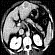
\includegraphics[width=0.6\linewidth]{celdas/tomo2-10-0}
  \caption{Tamaño de celda 10}
\end{subfigure}%
\begin{subfigure}{0.4\linewidth}
  \centering
  
\includegraphics[width=0.6\linewidth]{celdas/tomo2-13-0}
  \caption{Tamaño de celda 13}
\end{subfigure}
\begin{subfigure}{0.4\linewidth}
  \centering
  
\includegraphics[width=0.6\linewidth]{celdas/tomo2-17-0}
  \caption{Tamaño de celda 17}
\end{subfigure}%
\begin{subfigure}{0.4\linewidth}
  \centering
  
\includegraphics[width=0.6\linewidth]{celdas/tomo2-20-0}
  \caption{Tamaño de celda 20}
\end{subfigure}%

\begin{subfigure}{0.4\linewidth}
  \centering
  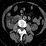
\includegraphics[width=0.6\linewidth]{celdas/tomo3-10-0}
  \caption{Tamaño de celda 10}
  \label{fig:muestras_celdas_tomo3_10}
\end{subfigure}%
\begin{subfigure}{0.4\linewidth}
  \centering
  
\includegraphics[width=0.6\linewidth]{celdas/tomo3-13-0}
  \caption{Tamaño de celda 13}
\end{subfigure}
\begin{subfigure}{0.4\linewidth}
  \centering
  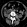
\includegraphics[width=0.6\linewidth]{celdas/tomo3-17-0}
  \caption{Tamaño de celda 17}
\end{subfigure}%
\begin{subfigure}{0.4\linewidth}
  \centering
  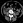
\includegraphics[width=0.6\linewidth]{celdas/tomo3-20-0}
  \caption{Tamaño de celda 20}
\end{subfigure}%

\caption{Imágenes \texttt{tomo2.csv} y \texttt{tomo3.csv} reconstruidas con diferentes tamaños de celda, nivel de ruido 0.0 y 20000 rayos aleatorios.}
\label{fig:muestras_celdas}
\end{figure}

%------------ Imagenes obtenidas con rayos VHD (verticales, horizontales y diagonales) ------------%

\begin{figure}
\centering
\begin{subfigure}{0.4\textwidth}
  \centering
  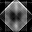
\includegraphics[width=0.6\linewidth]{rayos/phantom-vhd}
  \caption{\texttt{phantom.csv}, con tamaño de celda 8}
\end{subfigure}%
\begin{subfigure}{0.4\textwidth}
  \centering
  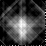
\includegraphics[width=0.6\linewidth]{rayos/tomo3-vhd}
  \caption{\texttt{tomo3.csv}, con tamaño de celda 10}
\end{subfigure}
\caption{Imágenes \texttt{phantom.csv} y \texttt{tomo3.csv} reconstruidas con rayos horizontales, verticales y diagonales. Nivel de ruido 0.0.}
\label{fig:muestras_vhd}
\end{figure}

%------------ Imagenes obtenidas con barridos ------------%

\begin{figure}
\centering
\begin{subfigure}{0.4\textwidth}
  \centering
  
\includegraphics[width=0.6\linewidth]{rayos/phantom-barrido}
  \caption{\texttt{phantom.csv}, con tamaño de celda 8}
\end{subfigure}%
\begin{subfigure}{0.4\textwidth}
  \centering
  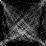
\includegraphics[width=0.6\linewidth]{rayos/tomo3-barrido}
  \caption{\texttt{tomo3.csv}, con tamaño de celda 10}
\end{subfigure}
\caption{Imágenes \texttt{phantom.csv} y \texttt{tomo3.csv} reconstruidas con rayos que barren la imagen desde las cuatro esquinas. Nivel de 
ruido 0.0.}
\label{fig:muestras_barrido}
\end{figure}

%------------ Imagenes obtenidas con metodo completo ------------%

\begin{figure}
\centering
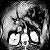
\includegraphics[width=0.3\linewidth]{rayos/tomo-completo}
\caption{Imagen \texttt{tomo.csv} reconstruida con el método ``completo'', tamaño de celda 2 y nivel de ruido 0.0.}
\label{fig:muestra_completo}
\end{figure}

%------------ Grafico que muestra PSNR en funcion de cantidad de rayos aleatorios ------------%

\begin{figure}[h]
\centering
\begin{tikzpicture}
\begin{axis}[
    title={PSNR en función de la cantidad de rayos aleatorios},
    xlabel={Cantidad de rayos aleatorios},
    ylabel={PSNR},
    xmin=0, xmax=7000,
    ymin=8, ymax=22,
    xtick={0,1000,2000,3000,4000,5000,6000,7000},
    ytick={8,10,12,14,16,18,20,22},
    legend pos=south east,
    ymajorgrids=true,
    % xmajorgrids=true,
    grid style=dashed,
]
 
\addplot[
    color=blue,
    % mark=*,
    % style=dashed,
    ]
    coordinates {
    (1444,15.7564)
    (2000,15.9915)
    (2500,17.2767)
    (3000,19.0018)
    (3500,19.9412)
    (4000,20.1737)
    (4500,20.6685)
    (5000,20.8324)
    (5500,21.0253)
    (6000,21.1197)
    (6500,21.1539)
    (7000,21.2395)
    };
    \addlegendentry{\texttt{tomo3.csv}}

\addplot[
    color=red,
    % mark=*,
    % style=dashed,
    ]
    coordinates {
    (676,8.41618)
    (1000,11.3252)
    (1500,15.016 )
    (2000,15.6017)
    (2500,16.1013)
    (3000,16.2221)
    (3500,16.3056)
    (4000,16.3317)
    (4500,16.3707)
    (5000,16.4363)
    (5500,16.4824)
    (6000,16.4942)
    (6500,16.5166)
    (7000,16.5248)
    };
    \addlegendentry{\texttt{phantom.csv}}

\end{axis}
\end{tikzpicture}
\caption{PSNR en función de cantidad de rayos aleatorios, para las imágenes \texttt{tomo3.csv} y \texttt{phantom.csv}, tamaños de celda 
12 y 10 respectivamente, y nivel de ruido 0.0.}
\label{fig:psnr_vs_aleats}
\end{figure}

%------------ Grafico que muestra nro cond en funcion de cantidad de rayos aleatorios ------------%

\begin{figure}[h]
\centering
\begin{tikzpicture}
\begin{axis}[
    title={$\kappa(D^tD)$ en función de la cantidad de rayos aleatorios},
    xlabel={Cantidad de rayos aleatorios},
    ylabel={$\kappa(D^tD)$},
    xmin=0, xmax=7000,
    ymin=0, ymax=36000,
    xtick={0,1000,2000,3000,4000,5000,6000,7000},
    ytick={0,5000,10000,15000,20000,25000,30000,35000},
    legend pos=north east,
    ymajorgrids=true,
    % xmajorgrids=true,
    grid style=dashed,
]
 
\addplot[
    color=blue,
    % mark=*,
    % style=dashed,
    ]
    coordinates {
    (2500,35281.5)
    (3000,22873)
    (3500,4247.11)
    (4000,2171.75)
    (4500,1884.09)
    (5000,1443.61)
    (5500,1115.55)
    (6000,1155.68)
    (6500,775.142)
    (7000,707.507)
    };
    \addlegendentry{\texttt{tomo3.csv}}

\addplot[
    color=red,
    % mark=*,
    % style=dashed,
    ]
    coordinates {
    (1500,11736.9)
    (2000,8422.15)
    (2500,964.307)
    (3000,550.485)
    (3500,442.103)
    (4000,341.59)
    (4500,317.157)
    (5000,300.344)
    (5500,290.834)
    (6000,283.758)
    (6500,276.984)
    (7000,265.96)
    };
    \addlegendentry{\texttt{phantom.csv}}

\end{axis}
\end{tikzpicture}
\caption{$\kappa(D^tD)$ en función de cantidad de rayos aleatorios, para las imágenes \texttt{tomo3.csv} y \texttt{phantom.csv}, tamaños de celda 
12 y 10 respectivamente, y nivel de ruido 0.0.}
\label{fig:ncond_vs_aleats}
\end{figure}

%------------ Imagenes obtenidas con rayos aleatorios ------------%

\begin{figure}
\centering
\begin{subfigure}{0.4\linewidth}
  \centering
  
\includegraphics[width=0.6\linewidth]{rayos/tomo3-aleat1444}
  \caption{1444 rayos aleatorios ($D$ resulta cuadrada).}
\end{subfigure}%
\begin{subfigure}{0.4\linewidth}
  \centering
  
\includegraphics[width=0.6\linewidth]{rayos/tomo3-aleat2500}
  \caption{2500 rayos aleatorios.}
\end{subfigure}
\begin{subfigure}{0.4\linewidth}
  \centering
  
\includegraphics[width=0.6\linewidth]{rayos/tomo3-aleat4000}
  \caption{4000 rayos aleatorios.}
\end{subfigure}%
\begin{subfigure}{0.4\linewidth}
  \centering
  
\includegraphics[width=0.6\linewidth]{rayos/tomo3-aleat7000}
  \caption{7000 rayos aleatorios.}
\end{subfigure}%

\begin{subfigure}{0.4\linewidth}
  \centering
  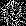
\includegraphics[width=0.6\linewidth]{rayos/phantom-aleat676}
  \caption{676 rayos aleatorios ($D$ resulta cuadrada).}
\end{subfigure}%
\begin{subfigure}{0.4\linewidth}
  \centering
  
\includegraphics[width=0.6\linewidth]{rayos/phantom-aleat1500}
  \caption{1500 rayos aleatorios.}
\end{subfigure}
\begin{subfigure}{0.4\linewidth}
  \centering
  
\includegraphics[width=0.6\linewidth]{rayos/phantom-aleat4000}
  \caption{4000 rayos aleatorios.}
\end{subfigure}%
\begin{subfigure}{0.4\linewidth}
  \centering
  
\includegraphics[width=0.6\linewidth]{rayos/phantom-aleat7000}
  \caption{7000 rayos aleatorios.}
\end{subfigure}%

\caption{Imágenes \texttt{tomo3.csv} y \texttt{phantom.csv} reconstruidas con tamaños de celda 12 y 10 respectivamente, nivel de ruido 0.0. Se 
muestran resultados para diferentes cantidades de rayos aleatorios.}
\label{fig:muestras_aleat}
\end{figure}

%---------- PSNR en funcion de ruido ----------%

\begin{figure}[h]
\centering
\begin{tikzpicture}
\begin{axis}[
    title={PSNR en función del nivel de ruido},
    xlabel={Nivel de ruido},
    ylabel={PSNR},
    xmin=0, xmax=20000,
    ymin=11, ymax=18,
    xtick={0,2000,4000,6000,8000,10000,12000,14000,16000,18000,20000},
    ytick={11,12,13,14,15,16,17,18},
    legend pos=south west,
    ymajorgrids=true,
    % xmajorgrids=true,
    grid style=dashed,
]
 
\addplot[
    color=blue,
    % mark=*,
    % style=dashed,
    ]
    coordinates {
    (0, 17.3091)
    (250,17.3067)
    (500,17.3023)
    (750,17.2877)
    (1000,17.2651)
    (1250,17.2518)
    (1500,17.2267)
    (1750,17.2191)
    (2000,17.1525)
    (2250,17.1179)
    (2500,17.0655)
    (2750,17.0334)
    (3000,16.96)
    (3250,16.8747)
    (3500,16.8909)
    (3750,16.8216)
    (4000,16.7531)
    (4250,16.7148)
    (4500,16.6147)
    (4750,16.529)
    (5000,16.4476)
    (5250,16.3861)
    (5500,16.3223)
    (5750,16.1855)
    (6000,16.0697)
    (6250,16.0754)
    (6500,15.9512)
    (6750,15.8443)
    (7000,15.8042)
    (7250,15.7652)
    (7500,15.6609)
    (7750,15.454)
    (8000,15.407)
    (8250,15.2654)
    (8500,15.1496)
    (8750,15.1083)
    (9000,15.0599)
    (9250,14.9569)
    (9500,14.8081)
    (9750,14.7154)
    (10000, 14.587)
    (10500, 14.5426)
    (11000, 14.2761)
    (11500, 14.1894)
    (12000, 14.0327)
    (12500, 13.8666)
    (13000, 13.6129)
    (13500, 13.5144)
    (14000, 13.2077)
    (14500, 13.1337)
    (15000, 12.9271)
    (15500, 12.7269)
    (16000, 12.5547)
    (16500, 12.5602)
    (17000, 12.1882)
    (17500, 12.1494)
    (18000, 11.9452)
    (18500, 11.6838)
    (19000, 11.7889)
    (19500, 11.5614)
    (20000, 11.4249)
    };
    \addlegendentry{\texttt{tomo2.csv}}

\end{axis}
\end{tikzpicture}
\caption{PSNR en función del nivel de ruido agregado a los tiempos de los rayos, para la imagen \texttt{tomo2.csv}, tamaño de celda 
10 con 20000 rayos aleatorios.}
\label{fig:psnr_vs_ruido}
\end{figure}

%----------- Imagenes obtenidas con varios niveles de ruido -----------%

\begin{figure}
\centering
\begin{subfigure}{0.4\linewidth}
  \centering
  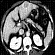
\includegraphics[width=0.6\linewidth]{ruido/tomo2-ruido0}
  \caption{Nivel de ruido: 0.}
\end{subfigure}
\begin{subfigure}{0.4\linewidth}
  \centering
  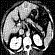
\includegraphics[width=0.6\linewidth]{ruido/tomo2-ruido4000}
  \caption{Nivel de ruido: 4000.}
\end{subfigure}
\begin{subfigure}{0.4\linewidth}
  \centering
  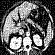
\includegraphics[width=0.6\linewidth]{ruido/tomo2-ruido8000}
  \caption{Nivel de ruido: 8000.}
\end{subfigure}
\begin{subfigure}{0.4\linewidth}
  \centering
  
\includegraphics[width=0.6\linewidth]{ruido/tomo2-ruido12000}
  \caption{Nivel de ruido: 12000.}
\end{subfigure}
\begin{subfigure}{0.4\linewidth}
  \centering
  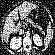
\includegraphics[width=0.6\linewidth]{ruido/tomo2-ruido16000}
  \caption{Nivel de ruido: 16000.}
\end{subfigure}
\begin{subfigure}{0.4\linewidth}
  \centering
  
\includegraphics[width=0.6\linewidth]{ruido/tomo2-ruido20000}
  \caption{Nivel de ruido: 20000.}
\end{subfigure}
\caption{Imagen \texttt{tomo2.csv} reconstruida con tamaño de celda 10 y 20000 rayos aleatorios. Se 
muestran resultados para diferentes niveles de ruido.}
\label{fig:muestras_ruido}
\end{figure}


\clearpage

\section{Discusión}

\subsection{Tamaño de celda}

Tal como se esperaba, en la Figura \ref{fig:psnr_vs_celda_1} observamos que el PSNR es mayor cuando las celdas son más chicas, o dicho de otra 
manera, cuanto las imágenes originales son divididas en más celdas. Esta propiedad es independiente de la imagen en cuestión, puesto que lo 
observamos tanto para \texttt{tomo2.csv} como para \texttt{tomo3.csv}. De más está decir que la Figura \ref{fig:muestras_celdas} muestra claramente 
las diferencias de calidad.

Un aspecto positivo es que a mayor tamaño de celda la reconstrucción es ciertamente de menor calidad, pero sin embargo la apariencia, a grandes 
rasgos, de la imagen reconstruida no cambia. Podría haber sucedido que al aumentar levemente el tamaño de celda la distribución de las intensidades 
cambiara, generando que zonas que antes eran oscuras ya no lo sean y viceversa; sin embargo no es este el caso, y es por esto que el PSNR tampoco 
disminuye abruptamente. Este resultado está fuertemente ligado al método de generación de rayos utilizado, que estudiaremos posteriormente.

En la Figura \ref{fig:ncond_vs_celda_1} observamos que no parece haber correlación entre el número de condición de $D^tD$ y el tamaño de las celdas. 
Muy al contrario, el valor de $\kappa(D^tD)$ tiene ``saltos'' repentinos cuando vemos distintos tamaños de celda. Podemos pensar que dicho parámetro 
no influye fuertemente en la forma que adquirirá la matriz (a excepción de su tamaño, por supuesto) y en su proximidad a una matriz singular, 
a diferencia de la forma de generación de rayos, que como veremos posteriormente, juega un rol importante en este aspecto.

\subsection{Rayos verticales, horizontales y diagonales}

En la Figura \ref{fig:muestras_vhd} observamos con claridad que las reconstrucciones están lejos de ser aceptables. En cada caso la distribución de 
intensidades respeta en cierto grado la de la imagen original, en el sentido de que, por ejemplo, para \texttt{tomo3.csv}, el área del centro es 
notablemente más clara que el resto, tal como en la imagen real. Sin embargo no se logran recuperar las formas de cada parte de la imagen ya que 
las reconstrucciones son muy difusas.

Si prestamos más atención se observa la aparición de ciertas rectas difusas con direcciones verticales, horizontales y diagonales de pendiente uno, 
tal como los rayos generados, y que parecerían seccionar la imagen. Podemos concluir que, debido a cómo armamos los rayos, solo se detectan cambios 
abruptos de las intensidades de los píxeles en estas tres direcciones, y es esa la razón por la cuál observamos estas rectas. Dicho de otra manera,
al irradiar la imagen en solo tres direcciones no estamos capturando la variación de densidad en otras direcciones.

Esto constituye un claro indicio de que los mejores métodos de generación de rayos serán aquellos que generen la mayor variedad de direcciones, 
siempre y cuando se logren atravesar la mayor cantidad de píxeles posibles.

La diferencia de calidad puede corroborarse con el PSNR obtenido. Por ejemplo, si miramos el PSNR obtenido al reconstruir \texttt{tomo3.csv} con 
tamaño de celda 10 y rayos aleatorios, en el gráfico de la Figura \ref{fig:psnr_vs_celda_1}, vemos que que está entre 21 y 22, mientras que el 
PSNR obtenido con rayos verticales, horizontales y diagonales es 17.0948.

Para \texttt{phantom.csv} y \texttt{tomo3.csv} la cantidad total de rayos generados en este caso fueron 1530 y 2706 respectivamente, que son mayores 
a la cantidad de celdas, 1024 y 2116. Sin embargo, nuestra implementación del método de la potencia devolvió únicamente 183 y 283 autovalores 
y autovectores para la matriz $D^tD$. Lo que sucede es que $D^tD$ no tiene rango completo en ninguno de los dos casos y por lo tanto $\kappa(D^tD)$ 
no está definido.

Para corroborar esto se guardó la matriz $D^tD$ de \texttt{phantom.csv} en un archivo aparte, y con un script de Python se obtuvieron sus 
autovalores ordenados con la función \texttt{eigh} de la biblioteca Numpy. En efecto, se comprobó que el autovalor número 183 era 
\texttt{2.79957053e+02}, mientras que el siguiente era \texttt{16308375e-11}, que es tan bajo que puede considerarse cero. Esto no fue exactamente 
así para el caso de \texttt{tomo3.csv}, dado que se pudo comprobar que existían unas decenas más de autovalores no nulos, y que nuestra 
implementación falló en calcular. Sin embargo, la mayoría de los autovalores de $D^tD$ en este caso también resultaron nulos, por eso es que tampoco 
tiene rango completo.

Concluimos entonces que esta forma de emitir rayos es propensa a generar una matriz $D^tD$ singular, lo cual implica que las soluciones obtenidas 
serán muy inestables.

\subsection{Rayos que barren la imagen}

Este caso es muy similar al anterior, en el sentido de que los fenómenos observados son los mismos. En la Figura \ref{fig:muestras_barrido} 
nuevamente observamos resultados inaceptables, y también vemos, sobretodo para \texttt{tomo3.csv}, rectas difusas que se asemejan a los rayos 
generados.

En este caso podemos afirmar que sí existen más direcciones que en el caso anterior, donde sólo había tres. Sin embargo, todos los rayos parten de 
cuatro posibles puntos, que son las esquinas de la imagen, y esto genera que la variedad de direcciones sea insuficiente para cada 
celda (por ejemplo, no existe ningún rayo vertical y horizontal que divida la imagen en dos partes). Esto explica los defectos observados.

Los valores de PSNR son incluso peores que los obtenidos con rayos verticales, horizontales y diagonales, marcando una desventaja frente al caso 
anterior.

Para \texttt{phantom.csv} no se pudieron calcular todos los autovalores, solo se calcularon 790. Con Numpy se verificó que el número de condición 
de $D^tD$ es muy alto, 1578918. Para \texttt{tomo3.csv} solo se obtuvieron 1088 autovalores, y también se verificó el número de condición con Numpy, 
que resultó ser 6470105.

Si bien las matrices $D^tD$ no resultaron singulares como antes, $\kappa(D^tD)$ resulta muy alto y por ende las soluciones son más inestables.

\subsection{Rayos aleatorios y método completo}

En la Figura \ref{fig:psnr_vs_aleats} observamos que el PSNR obtenido mejora al aumentar la cantidad de rayos aleatorios, para ambas imágenes. Para 
\texttt{tomo3.csv} el PSNR obtenido con 7000 rayos es prácticamente igual al obtenido con 20000 rayos, como se observa en la Figura 
\ref{fig:psnr_vs_celda_1}. Esto indica que la velocidad de crecimiento del PSNR disminuye a medida que la cantidad de rayos aleatorios aumenta.

En la Figura \ref{fig:muestras_aleat} vemos cómo aumenta la calidad, según la propia percepción humana, a mayor cantidad de rayos. En las 
reconstrucciones defectuosas se puede notar un cierto efecto de ruido, es decir, hay píxeles que resultan muy blancos y otros muy oscuros, sin 
seguirse ningún patrón en particular. Lo importante es que casi todas las imágenes (siendo la reconstrucción de \texttt{phantom.csv} con 676 rayos 
una clara excepción) se asemejan mucho a la original, principalmente porque no encontramos los defectos que surgen con los otros dos métodos de 
generación de rayos. No solo coinciden en gran medida las intensidades, si no que las formas y los bordes de cada parte de la imagen original son 
recuperados con considerable precisión.

Esto se debe a que ahora sí resulta que cada celda es atravesada por muchos rayos en diferentes direcciones. Esta variedad en los recorridos de los 
rayos permite capturar la mayor información de la imagen original, teniendo en cuenta las variaciones de las intensidades de los píxeles en todas 
las direcciones. Por supuesto, si no proporcionamos la cantidad suficiente de rayos, la reconstrucción será más defectuosa, tal como pudimos 
observar. Pero estos defectos no son más que intensidades erróneas en píxeles aleatorios de la imagen.

Otro resultado que mejora cuando aumenta la cantidad de rayos es el número de condición de $D^tD$. En la Figura \ref{fig:ncond_vs_aleats} podemos 
observar que disminuye abruptamente 
al principio, sin embargo, una vez que empezamos a generar más de 4000 rayos parece estabilizarse, es decir, la velocidad de decrecimiento tiende 
a ser cero. Por lo tanto podemos concluir que a mayor cantidad de rayos aleatorios, más estable será la solución obtenida, indepenidentemente del 
nivel de ruido utilizado.

En la Figura \ref{fig:muestra_completo} podemos ver la imagen \texttt{tomo.csv} reconstruida con el método completo de generación de rayos. 
En este caso todo rayo que viaje de un lado de la imagen al lado opuesto es generado. Es claro que el requisito que ya sabemos que debe cumplirse 
---que cada celda sea atravesada por muchos rayos con diversas direcciones--- se cumple para este método. Y es natural que la imagen obtenida 
sea bastante precisa, como con el método aleatorio. Sin embargo, la clara desventaja es que la cantidad de rayos a generar puede llegar a ser masiva 
con una imagen como \texttt{tomo2.csv} o \texttt{tomo3.csv}. Esto implica serias consecuencias en cuanto al tiempo de procesamiento y a la memoria 
utilizada por el programa. Por eso es que concluimos que el método aleatorio es superior, con el cual se pueden obtener resultados casi idénticos 
con muchos menos rayos. Además, el número de condición $\kappa(D^tD)$ en este caso resultó ser 10052, un valor bastante alto. De todas formas sería 
necesario probar este método con imágenes de diferentes tamaños para poder afirmar algo sobre cómo influye en el número de condición, pero resulta 
muy complicado debido a los inconvenientes recién mencionados.

\subsection{Nivel de ruido}

En la Figura \ref{fig:psnr_vs_ruido} observamos que el PSNR empieza variando un poco para los primeros niveles de ruido, sin embargo, luego del 
nivel 3000 aproximadamente, el PSNR comienza a decrecer linealmente, indicando que las reconstrucciones son cada vez más erróneas.

Según los resultados de la Figura \ref{fig:muestras_ruido}, el efecto producido es similar al que observamos cuando probamos reconstrucciones con 
escasos rayos aleatorios, a pesar de que ahora estamos estudiando un parámetro completamente diferente y que no influye en la matriz $D$. Vemos que 
a medida que el nivel de ruido aumenta surgen píxeles distribuidos uniformemente en toda la imagen cuyas intensidades no coinciden con las de los 
píxeles que los rodean.

Esto era un comportamiento esperable dado que cada tiempo de rayo $t_k$ viene determinado por la suma de las intensidades de todos los píxeles que 
atravesó. Si perturbamos un $t_k$ de manera aleatoria estaremos de alguna manera indicando que las intensidades de los píxeles atravesados por el 
rayo en cuestión son distintas de las de la imagen original, y como estas perturbaciones son independientes entre sí, no hay razón para creer que la 
imagen reconstruida cambiará de una manera particular. Al contrario, lo que sucede es que las intensidades de píxeles individuales cambian 
aleatoriamente.

Durante esta experiencia observamos qué tan grandes resultaron ser los tiempos $t_k$. Algunos resultaron un poco mayores a 100000, mientras que 
otros rondaban 30000. En cualquier caso, es claro que un nivel de ruido como 20000 es un nivel muy alto para este caso, puesto que en relación 
con los $t_k$ originales el cambio puede ser muy drástico. Sin embargo, en la imagen reconstruida no se perdió completamente la esencia de la imagen 
original. Para niveles de ruido más bajos, como 4000, que resultan más razonables si pensamos en mediciones reales, el impacto del ruido es mínimo.

Lo que influye notoriamente en este aspecto es el número de condición de $D^tD$, puesto que dicho valor determina qué tanta variación habrá 
entre dos soluciones $s_1$ y $s_2$ de los sistemas $D^tDs = D^tt_1$ y $D^tDs = D^tt_2$ respectivamente, siendo $t_1$ cercano a $t_2$. Notemos que 
ambos sistemas son ecuaciones normales asociadas a dos problemas de cuadrados mínimos $Ds = t_1$ y $Ds = t_2$. Por lo tanto, con un número de 
condición de $D^tD$ muy alto las soluciones al problema de cuadrados mínimos típicamente serán muy diferentes ante pequeñas perturbaciones en los 
tiempos. Ya vimos que con el método de generación de rayos aleatorios los valores de $\kappa(D^tD)$ tienden a ser más bajos que con otros métodos, 
y gracias a eso podemos observar en este caso que con niveles de ruido bajos las intensidades de los píxeles en la imagen reconstruida no 
cambian abruptamente.



\newpage

\section{Conclusión}

En primer lugar, es necesario remarcar que las tomografías computadas que se realizan a diario involucran un proceso muchísimo más complejo que el 
descripto en este trabajo. Por lo tanto, estableceremos las conclusiones del mismo entendiendo que el objetivo de los métodos propuestos es 
simular la emisión de rayos X sobre una imagen de manera simplificada, y con los datos obtenidos reconstruir la misma con la mayor precisión posible. 

En este sentido, es claro que la manera en que se emiten los rayos resulta decisiva a la hora de evaluar qué tan buena es la reconstrucción.
Vimos que el método de generación de rayos aleatorios resultó ser aquel que genera el sistema de ecuaciones más representativo, en comparación con 
los otros métodos propuestos. El hecho de que las celdas de la imagen sean atravesadas por varios rayos y en diversas direcciones resultó ser lo 
que diferencia a este método del resto, ya que permitió obtener reconstrucciones donde se preserva bien la distribución de las intensidades de los 
píxeles y las formas de las distintas partes de la imagen original.

El tamaño de celda elegido para la discretización es sin dudas un parámetro decisivo. Celdas muy chicas garantizan una mejor calidad de la imagen 
generada, pero se debe decidir hasta qué punto uno está dispuesto a sacrificar velocidad de procesamiento por calidad.

La descomposición SVD de $D$ resulta apropiada para hallar fácilmente la solución de cuadrados mínimos del sistema $Ds=t$, puesto que no implica 
que se deban realizar cálculos numéricamente inestables, suponiendo que ya contamos con la descomposición. Sin embargo, es necesario contar con un 
método eficaz para la obtención de los autovalores y autovectores de $D^tD$ (o $DD^t$). El método de la potencia con deflación no es la mejor opción 
ya que no solo es poco eficiente en cuanto a tiempo de procesamiento, si no que además requiere el cumplimiento 
de ciertas hipótesis y puede haber un considerable arrastre de error en los cálculos, debido a los problemas comunes de la aritmética finita.
En el desarrollo del trabajo propusimos un método que logra en cierta medida paliar estos problemas que pueden surgir, sin descuidar el rendimiento, 
sin embargo está lejos de ser perfecto.

A continuación enunciamos posibles extensiones que podrían hacerse:

\begin{itemize}
\item Obtención de autovalores y autovectores con otro algoritmo.
\item En vez de utilizar la descomposición SVD, hallar la solución de cuadrados mínimos resolviendo las ecuaciones normales mediante las 
factorizaciones QR y Cholesky de $D^tD$, los métodos iterativos de Jacobi y Gauss-Seidel, y eliminación gaussiana.
\item Nuevos métodos de generación de rayos.
\end{itemize}

Para finalizar, concluimos que teniendo un buen método de generación de rayos, la aproximación de la solución mediante cuadrados mínimos constituye 
un método muy efectivo que permite obtener reconstrucciones satisfactorias de la imagen original.


% Los resultados obtenidos con el método primer método de generación de rayos son los siguientes:

% \begin{itemize}
% \item \texttt{phantom.csv} con tamaño de celda 8, nivel de ruido 0.0: PSNR = 14.7697, $\kappa{D^tD}$ = 3494.38.
% \item \texttt{tomo3.csv} con tamaño de celda 10, nivel de ruido 0.0: PSNR = , $\kappa{D^tD}$ = .
% \end{itemize}

% \begin{table}
% \begin{tabular}{|l|l|l|l|l|l|l|} 
% \hline
% Rango:            & [0.1, 0.9] & [0.01, 0.5] & [0.4, 0.6] & [0.1, 0.5] & [0.6, 1.0] & [0.5, 1.0]  \\ 
% \hline
% \textit{Accuracy} & 0.606      & 0.7         & 0.595      & 0.662      & 0.6        & 0.603       \\
% \hline
% \end{tabular}
% \caption{Hola}
% \end{table}


\newpage

\section{Apéndice}

\subsection*{A: Enunciado del TP}

\includegraphics[scale=0.75, page=1]{tp3.pdf}
\includepdf[page=2-, offset=75 -75]{tp3.pdf}

\subsection*{B: Demostraciones relevantes}

\begin{itemize}

\item Obtención de la solución de cuadrados mínimos del sistema $Ds = t$ mediante la descomposición SVD de $D$:

En primer lugar supondremos que $D \in \mathbb{R}^{n^2 \times m}$ es tal que $r = \text{rg}(D) < n^2$.

Se quiere minimizar $||Ds - t||^2$. Consideremos la descomposición SVD de $D$, $D = U\Sigma V^t$. Dado que $U^t$ es ortogonal:

\[
||Ds - t||^2 = ||U^t(U\Sigma V^t s - t)||^2 = ||\Sigma V^t s - U^tt||^2
\]

Dado que $V^t$ es inversible (por ser ortogonal), el problema de encontrar $s$ tal que minimice $||\Sigma V^t s - U^tt||^2$ es equivalente 
a encontrar $y \in \mathbb{R}^{n^2} = \text{Im}(V^t)$ tal que minimice $||\Sigma y - U^tt||^2$ y luego obtener $s = Vy$. Si escribimos:

\[
U^tt = 
    \begin{pmatrix}
      c \\
      d
    \end{pmatrix}
\]

\noindent con $c \in \mathbb{R}^{r}$ y $d \in \mathbb{R}^{m - r}$, entonces:

\[
||\Sigma y - U^tt||^2 = 
\left\lVert
\begin{pmatrix}
      \sigma_1 y_1 \\
      \vdots \\
      \sigma_r y_r \\
      0 \\
      \vdots \\
      0
\end{pmatrix}
-
\begin{pmatrix}
      c \\
      d
\end{pmatrix}
\right\rVert^2
=
\left\lVert
\begin{pmatrix}
    \sigma_1 y_1 - c_1 \\
    \vdots \\
    \sigma_r y_r - c_r \\
\end{pmatrix}
\right\rVert^2
+ ||d||^2
\]

\noindent donde $\sigma_1 \ldots \sigma_r$ son los valores singulares de $D$ (las entradas positivas de la diagonal principal de $\Sigma$). Si 
tomamos:

\[
y = 
    \begin{pmatrix}
      c_1/\sigma_1 \\
      \vdots       \\
      c_r/\sigma_r \\
      y_{r+1}      \\
      \vdots       \\
      y_{n^2}      
    \end{pmatrix}
\]

\noindent con $y_{r+1} \ldots y_{n^2}$ arbitrarios entonces se minimiza $||\Sigma y - U^tt||^2$. Entonces obtieniendo $s = Vy$ logramos minimizar 
$||\Sigma V^t s - U^tt||^2 = ||Ds - t||^2$.

Si $r = n^2$ entonces solo podremos obtener un único $y$ y por ende un único $s$, lo cual tiene sentido puesto que al ser $D$ de rango completo 
la solución de cuadrados mínimos es única.

\end{itemize}

% \newpage

% \begin{thebibliography}{}
% % \bibitem{art1}
% % Aprendizaje automático: \textit{https://es.wikipedia.org/wiki/Aprendizaje_automático}
% % \bibitem{art2}
% % Varianza: \textit{https://es.wikipedia.org/wiki/Varianza}
% % \bibitem{art3}
% % Matriz de covarianza: \textit{https://es.wikipedia.org/wiki/Matriz_de_covarianza}
% % \bibitem{art4}
% % Método de potencia: \textit{https://es.wikipedia.org/wiki/Método_de_las_potencias}
% % \bibitem{art5}
% % Beyer K., Goldstein J., Ramakrishnan R., Shaft U.: When is Nearest Neighbors
% % Meaningful? \textit{ICDT Conference Proceedings}, 1999.
% \end{thebibliography}

\end{document}
